\section{Ausgangslage}
\label{sec:Ausgangslage}

Die Basis für das Projekt 6 hat das Projekt 5 gebildet, in welchem ein Konzept erstellt wurde, welches die Hauptkomponenten der Maschine festlegte und deren Arbeitsweise. Aus dieser Entscheidungsfindung wurde dann ein Blockschaltbild erstellt, welches in Abbildung \ref{fig:P5_Blockschaltbild_Partymixer} zu sehen ist. Ein weiterer Teil des Projekt 5 war es, die gewählten Komponenten und die daraus entstandenen Teilsysteme in einem Testaufbau aufzubauen und zu evaluieren. Dazu gehörten die Speisungen (48V, 12V, 5V und 3.3V), der Mikrocontroller, das Display, der Motor, die Pumpenansteuerung und die Durchflussmessgeräte.

\begin{figure}[H]
\center
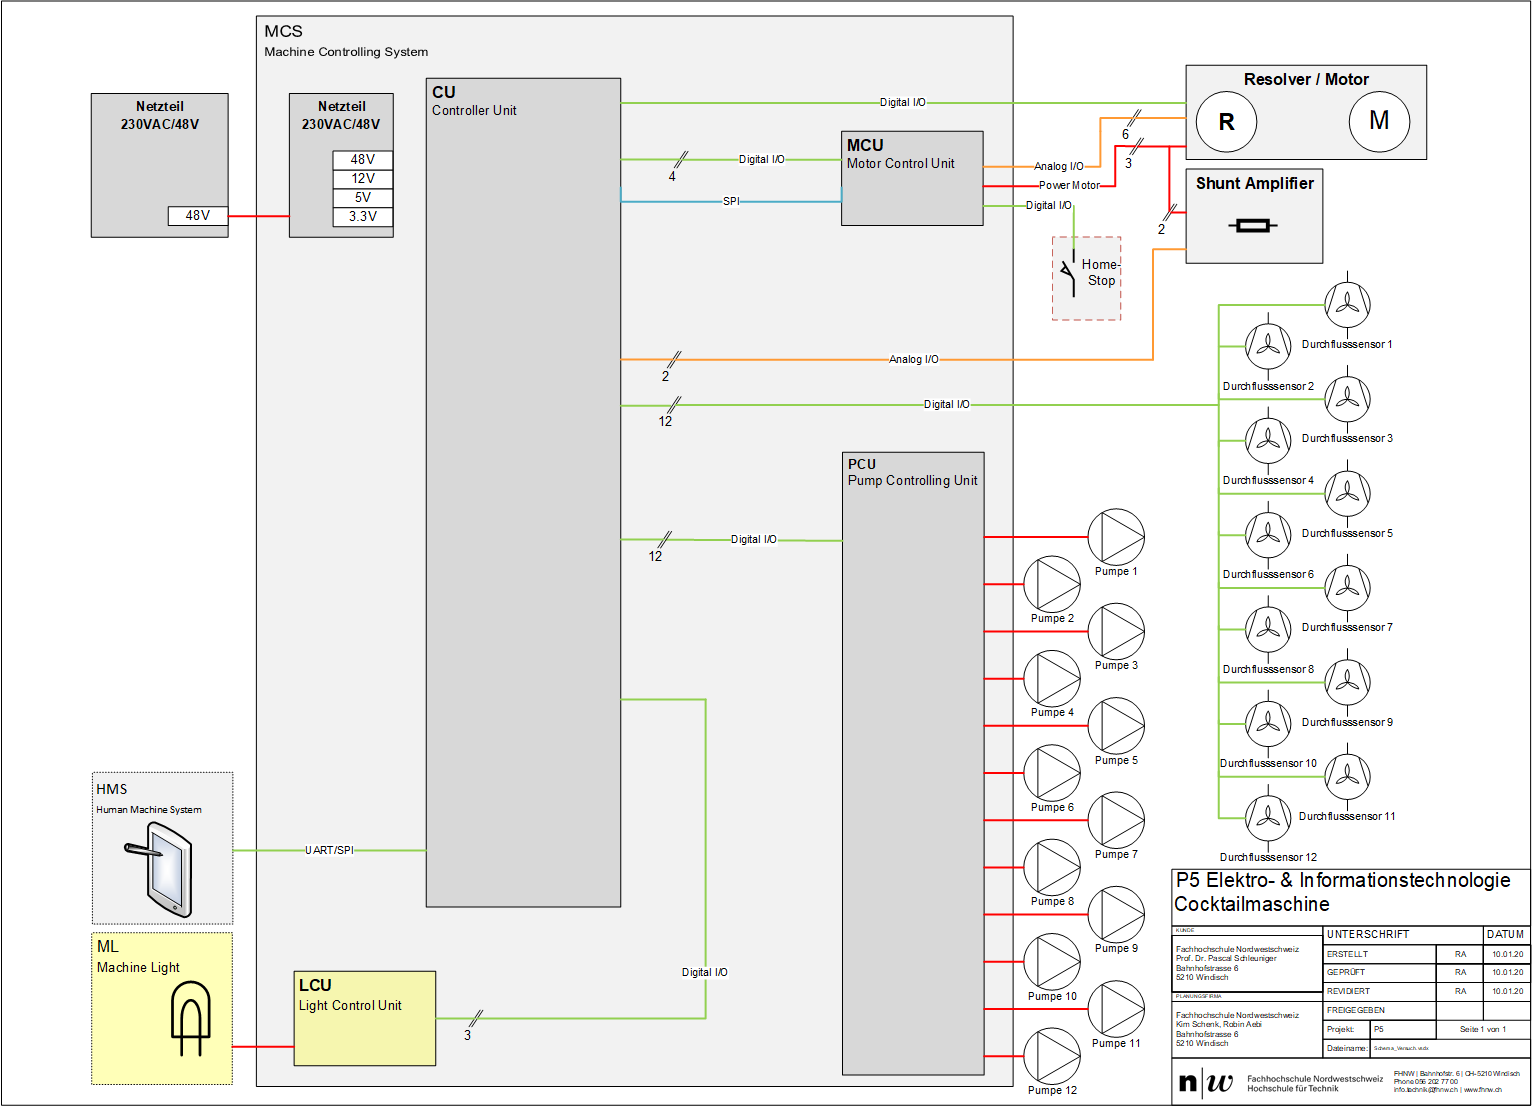
\includegraphics[angle=90, width = 0.82\textwidth]{graphics/P5-Blockschema}
\caption{Blockschaltbild des PartyMixer's gemäss Projekt 5.}
\label{fig:P5_Blockschaltbild_Partymixer}
\end{figure}

\newpage

